\chapter{Single-Stage Amplifiers}

%%%
\section{General Considerations}
从本章开始将进入模拟电路的部分。本章使用的符号如表 \ref{tab:chapter4-symbols} 所示。
\begin{table}[!htb]
    \centering
    \caption{Single-Stage Amplifiers Symbols}
    \label{tab:chapter4-symbols}
    \begin{NiceTabular}{cccc}
        \Xhline{1pt}
        \textbf{Symbol} & \textbf{Meaning} & \textbf{Unit} & \textbf{Polarity} \\ \hline
        $v_[in]$ & 输入电压(Input voltage) & $\unit{\volt}$ & $\diagdown$ \\
        $v_[out]$ & 输出电压(Output voltage) & $\unit{\volt}$ & $\diagdown$ \\
        $i_[in]$ & 输入电流(Input current) & $\unit{\ampere}$ & $\diagdown$ \\
        $i_[out]$ & 输出电流(Output current) & $\unit{\ampere}$ & $\diagdown$ \\
        $R_[in]$ & 输入电阻(Input resistance) & $\unit{\ohm}$ & + \\
        $Z_[in]$ & 输入阻抗(Input impedance) & $\unit{\ohm}$ & $\diagdown$ \\
        $R_[out]$ & 输出电阻(Output resistance) & $\unit{\ohm}$ & + \\
        $Z_[out]$ & 输出阻抗(Output impedance) & $\unit{\ohm}$ & $\diagdown$ \\
        $R_[load]/R_[L]$ & 负载电阻(Load resistance) & $\unit{\ohm}$ & + \\
        $Z_[load]/Z_[L]$ & 负载阻抗(Load impedance) & $\unit{\ohm}$ & $\diagdown$ \\
        $A_[v]$ & 电压增益(Voltage gain/Gain) & 1 & $\diagdown$ \\
        $G_[m]$ & 跨导(Transconductance) & $\unit{\siemens}$ & $\diagdown$ \\
        $g$ & 转移电导(Transfer conductance) & $\unit{\siemens}$ & $\diagdown$ \\
        \Xhline{1pt}
    \end{NiceTabular}
\end{table}

%%%%
\subsection{Equivalent of a One-Port Network}
首先回顾一下一端口电路的等效。对于一个线性含源一端口电阻电路,可以进行戴维宁等效(Thevenin Equivalent)或诺顿等效(Norton Equivalent)的转换,如图 \ref{fig:thevenin-norton-equivalent} 所示。
\begin{figure}[htp!]
    \centering
    \begin{subfigure}[b]{\textwidth}
        \centering
        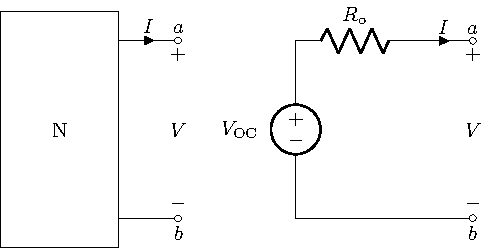
\includegraphics[]{thevenin.pdf}
        \caption{戴维宁等效}
    \end{subfigure}
    \begin{subfigure}[b]{\linewidth}
        \centering
        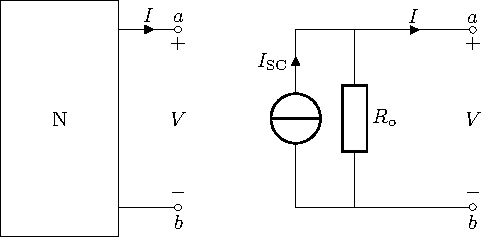
\includegraphics[]{norton.pdf}
        \caption{诺顿等效}
    \end{subfigure}
    \caption{戴维宁等效与诺顿等效}
    \label{fig:thevenin-norton-equivalent}
\end{figure}

在戴维宁等效中,$V_[OC]$为开路电压,$R_[o]$为将N内所有的独立源置零后两端钮间的等效电阻。在诺顿等效中,$I_[SC]$为短路电流,$R_[o]$同样为两端钮间的等效电阻。
它们具有关系$V_[OC] = I_[SC] \cdot R_[o]$。

%%%%
\subsection{Input and Output Impedances}
对于放大电路,我们通常会将其分为很多级,每一级都有输入和输出。为了简化,我们对其进行等效,如图 \ref{fig:input-output-impedance} 所示。
\begin{figure}[!htb]
    \centering
    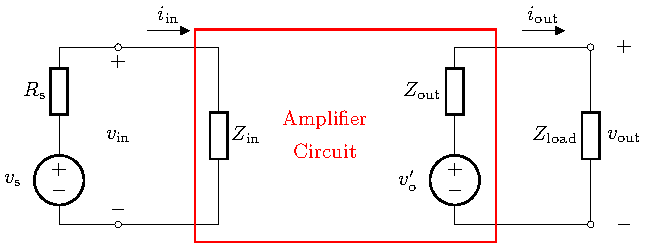
\includegraphics[]{input-output-impedance.pdf}
    \caption{放大电路示意图}
    \label{fig:input-output-impedance}
\end{figure}
需要注意,所谓的\textbf{放大电路,都是基于小信号而言的}。

\textbf{输入阻抗(Input Impedance)}$\bm{Z_{\mathrm{in}}}$是从放大电路输入端看进去的等效电阻,其值为输入端电压$v_[in]$与输入端电流$i_[in]$的比值,
\begin{equation}
    Z_[in] = \frac{v_[in]}{i_[in]}
\end{equation}
通常我们希望输入阻抗$Z_[in]$的值尽量大,这样才能使得放大电路从信号源索取的电流尽量小,降低功耗,同时使放大电路得到的输入电压$v_[in]$更接近信号源的输出电压$v_[s]$,信号电压的损失更小。

放大电路从输出端看进去,内部是一个含源一端口电路,可以等效为一个电压源与电阻串联或一个电流源与电阻并联。这个电阻就是\textbf{输出阻抗(Output Impedance)}$\bm{Z_{\mathrm{out}}}$,其值为将输入信号源置零后,输出端电压$v_[out0]$与输出端电流$i_[out0]$的比值,
\begin{equation}
    Z_[out] = \frac{v_[out0]}{i_[out0]}
\end{equation}
也可以用添加测试电流$I_[X]$或测试电压$V_[X]$的方式来测量输出阻抗。\\
通常我们希望输出阻抗$Z_[out]$的值尽量小,这样才能使得放大电路的负载能分到更大的电压,电路的带负载能力更强。

需要注意,输入阻抗是从输入端看去的,在等效电路中位于输出的位置,而输出阻抗是从输出端看去的,在等效电路中位于输入的位置。这在初学时容易记忆错误。
同时,\textcolor{red}{输入阻抗与输出阻抗之间\textbf{没有对称关系}},它们是两个不同的概念。

%%%%
\subsection{Basic Amplifier Analysis Principles}
在模拟集成电路设计中,各级放大电路一般都是基于 MOSFET 来实现的。而为了实现高的输入阻抗,一般又会采用\textbf{栅极作为输入端}。

结合 MOSFET 的小信号模型(图 \ref{fig:mosfet-small-signal-model}),我们通常使用图 \ref{fig:amplifier-equivalent-circuit} 所示的等效电路来进行分析计算。
\begin{figure}[h!tb]
    \centering
    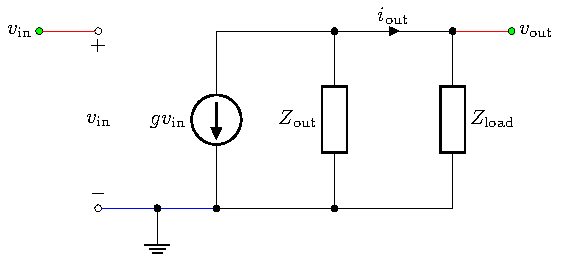
\includegraphics[]{amplifier-equivalent-circuit.pdf}
    \caption{放大电路等效电路}
    \label{fig:amplifier-equivalent-circuit}
\end{figure}
其中$g$为压控电流源(VCCS)的转移电导\footnote{转移电导$g$与放大电路的跨导$G_[m]$是两个不同的概念,转移电导是针对一个受控源而言的,而跨导是整个放大电路输出电流与输入电压的小信号比值。在JianJun Zhou的ppt中二者没有很好地区分,容易误解,在此指出。},$Z_[out]$为输出阻抗,$Z_[load]$为负载阻抗,$v_[in]$为输入电压,$v_[out]$为输出电压。

注意图 \ref{fig:amplifier-equivalent-circuit} 中的输入端的等效电源是一个受控源而不是独立源,但这并不是误用诺顿等效。这个受控源的电流是$g v_[in]$,转移电导$g$是由电路的静态工作点(大信号)决定的,而输入电压$v_[in]$是由上一级电路决定的,因此这个受控源的电流实际不受这一级小信号放大电路本身的影响,相对于当前的小信号电路是独立的,是一个“独立源”。

将单级放大电路简化为图 \ref{fig:amplifier-equivalent-circuit} 所示的形式后,容易看出其\textbf{增益(Gain)$A_[v]$}为
\begin{equation}
    A_[v] = \frac{v_[out]}{v_[in]} = -g (Z_[out] // Z_[load])
    \label{eq:amplifier-gain}
\end{equation}
式 \ref{eq:amplifier-gain} 非常重要,在后续的分析中会经常用到。有时我们在计算时会忽略负号,仅考虑增益的绝对值(电压放大的倍数)。

这里说明几个初学小信号电路图时令人困惑的问题(有些大信号电路图也有这些问题)。
\begin{itemize}
    \item \textbf{小信号输入和输出都是相对于地的}。小信号输入电压$v_[in]$和输出电压$v_[out]$都是相对于地的电压。很多时候在图中输入输出电压只接入了一个端钮,例如图 \ref{fig:amplifier-equivalent-circuit} 中的绿色端钮。我们应该知道另一个端钮是没有画出的接地点。

    \item \textbf{有些导线中是没有电流的,它只表示两个节点的电位相等}。很多时候,为了表示多个节点都接地,我们会用导线将这些节点相连避免在图中绘制多个接地点。这些导线中是没有电流的,它只表示两个节点的电位相等,在分析电流时可直接将其忽略。图 \ref{fig:amplifier-equivalent-circuit} 中的蓝色导线就是一个例子。

    \item \textbf{有些端钮是悬空的,只代表一个电压探针}。有些时候,为了简化图形,我们会将某些端钮悬空,引出一条悬空导线并给出一个电压值标签,代表一个电压探针。例如图 \ref{fig:amplifier-equivalent-circuit} 中的$v_[out]$。与探针相连的导线中是没有电流的,只是为了作图的方便引出一条导线。图 \ref{fig:amplifier-equivalent-circuit} 中的红色导线中是没有电流的。但需要注意,并不是所有这样的端钮都代表探针,例如一些大信号电路图中的$V_[DD]$就不是探针,它是一个电源,与其相连的导线中是有电流的。
\end{itemize}
这些特殊情况并不会在图中标出,需要我们自己去判断理解。

%%%%
\subsection{``Common'' What?}
在分析放大电路时,我们经常会遇到“共X放大电路”(Common Xxx)的概念,例如“共源放大电路”(Common Source Amplifier,CS Amplifier),“共栅放大电路”(Common Gate Amplifier,CG Amplifier),“共漏放大电路”(Common Drain Amplifier,CD Amplifier)等等。这里的“共”到底是什么意思呢?
